\section{Interface Design} % (fold)
\label{sec:interface_design}

The interface design was not a straightforward task, but rather an iterative process where several alternatives were weighted.
Constant feedback from other members of the project helped shaping it until getting to the final design.
At the end of this work two interfaces were fully designed to bring the same functionality under both desktop and mobile constraints.

\subsection{Redesign} % (fold)
\label{sub:redesign}

The previous design had several flaws that needed to be fixed.
Also, since more functionality were implemented, additional abstractions needed to be designed.
Considering these two facts, the main points behind this redesign were:

\begin{description}
  \item[Organization] The previous design was quite chaotic, the elements were just scattered and the visual impact was odd.
  By constraining the design to a grid, elements fall into place, so the user impression improves a lot.
  \item[Simplicity] For example, the previous background was a little distracting, and the colors gave more importance to the background than to the foreground elements.
  By simplifying the shapes and desaturating the colors, now elements are more easily recognizable.
  
  Also, buttons are easier to distinguish now, because they are bright orange while the rest of the interface is desaturated.
  All new images also follow this convention, so that they do not feel out of place.
  Another example is the new trash icon: it is desaturated by default, but when the user drags something onto that icon, it activates showing the full color version of that image.
  \item[Legibility] Some texts in the previous design were very difficult to read: white over very light orange, for example.
  In this design this was a concern, and it results in a high contrast color palette: white over black, black over white.
  Other design tricks also help with the contrast, like adding shadows in some texts labels.
  \item[Smoothness] Animations have been heavily used in the interface, to give the interface a responsive feeling to the user actions.
  For example, when the user drags the icon it slightly fades and when the mouse is over a valid container it turns opaque.
  
  Also, when the icon is released onto an invalid container or when a session is deleted/duplicated/transferred, the icon smoothly \emph{flies} from one point to another.
  These nice little touches are not just superfluous gimmicks, but they enhance the user experience.
  \item[Adaptability] The previous interface was static, all elements had fixed sizes and positions.
  Now, the elements are designed to be resized automatically to fit the available space.
  \item[Customizability] The user can now move and resize his devices, so there are new elements to make this task easier.
  When the mouse is over a device, two handles appear: one to move it and another one to resize it.
  The user just has to drag them to see how the devices change live.
  
  Another visual element added for resizing the sidebar is another handle, acting as a cue to the user.
  The two panes of the interface resize accordingly with the position of that knob.
  \item[Intuitiveness] For the user it makes more sense tagging the sessions with a still image from the video rather than with a generic icon.
  That is the most effective way to visually discriminate two different sessions.
  \item[Condensedness] On the one hand simplicity was one of our goals, but on the other hand more information will be added to the sidebar.
  This has been solved by adding \emph{tabs} to the sidebar so that the user can alternate between his buddy list and the new content list.
  
  Also, in the new content list an \emph{accordion} has been implemented to handle the different categories.
  So when content from one category is shown, the others are collapsed.
\end{description}

Figure~\ref{fig:pnai-buddies} shows how the new interface looks like, in contrast to the old interface showed in Figure~\ref{fig:pnai-old} (that figure only contains the main frame).
In that figure there are several obvious changes, new icons like the trash and buddies, new elements and the overall look.
However most of the same abstractions are used, like drawing sessions inside of the devices.

\begin{figure}[htbp]
  \centering
    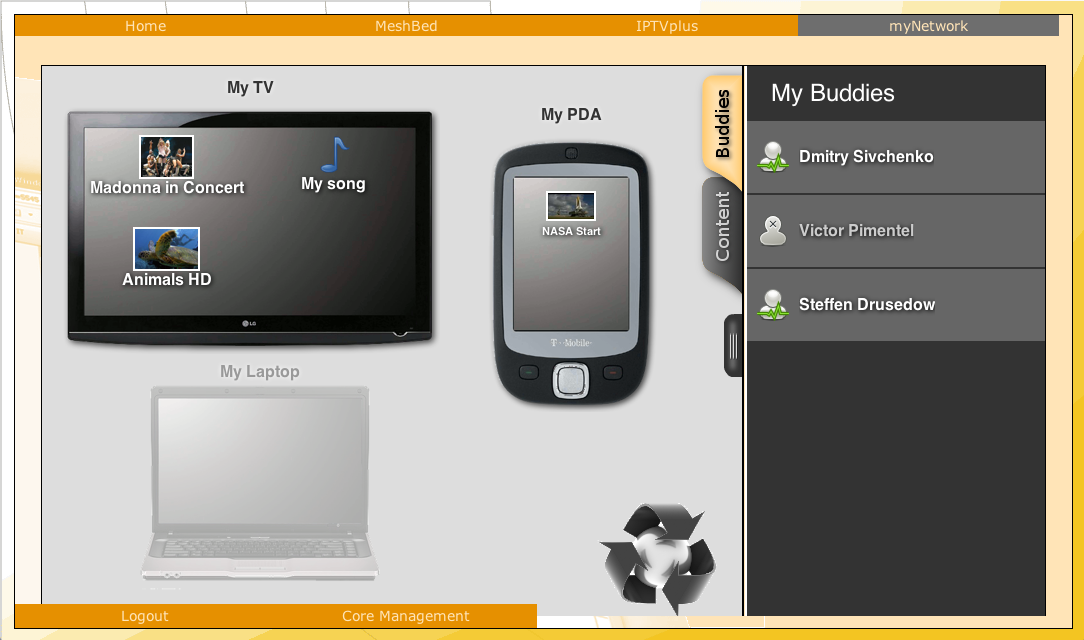
\includegraphics[width=\textwidth]{pnai-buddies}
  \caption{New PNAI interface}
  \label{fig:pnai-buddies}
\end{figure}

But now there are two tabs; the previous figure showing the buddy list like the old interface.
Figure~\ref{fig:pnai-content} exposes the second tab, the content list, that appears if the user clicks on the \emph{Content} tab.
This content list encloses all the information of the \idx{IPTVplus} page (see Figure~\ref{fig:iptvplus}) but without having to leave this page.
Initially the content list appears completely collapsed (Figure~\ref{fig:pnai-content-closed}) and then the user can click on any category and videos from that category will be shown (Figure~\ref{fig:pnai-content-open}).

\begin{figure}[htbp]
  \centering
  \subfigure[Initial view, categories are collapsed]{
    \label{fig:pnai-content-closed}
    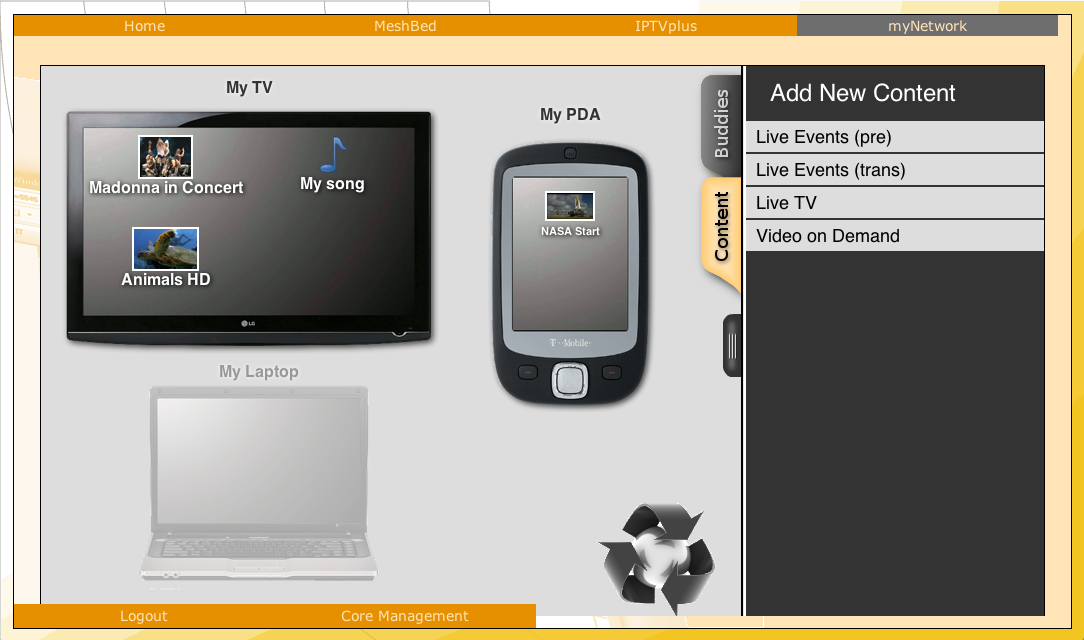
\includegraphics[width=\textwidth]{pnai-content}
  }
  \subfigure[User clicks on a category]{
    \label{fig:pnai-content-open}
    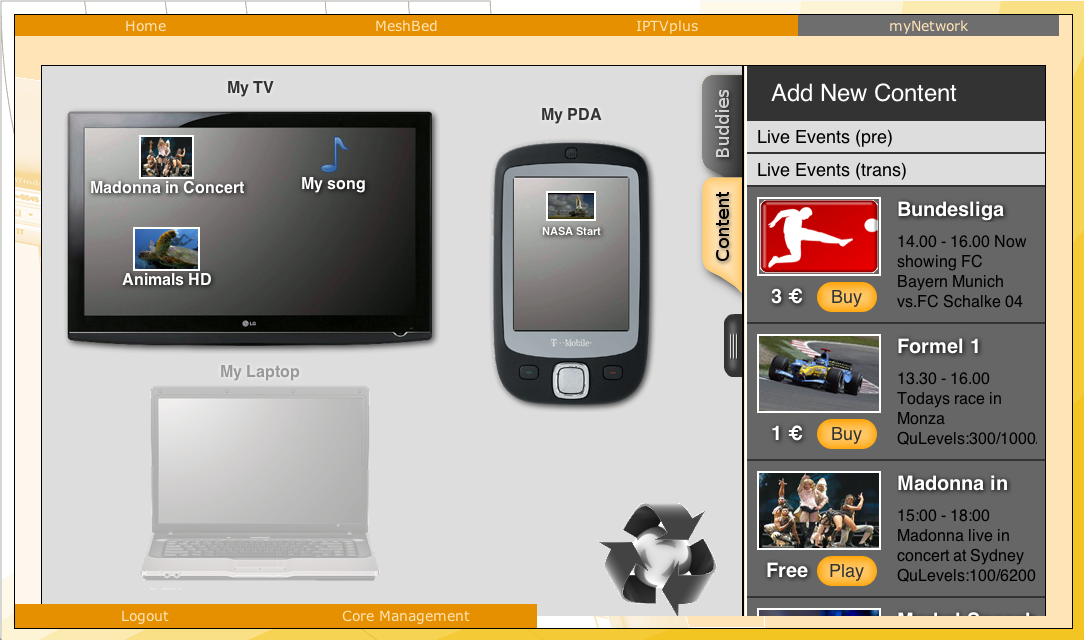
\includegraphics[width=\textwidth]{pnai-content-open}
  }
  \caption{New content sidebar}
  \label{fig:pnai-content}
\end{figure}

As explained before, the sidebar can be dynamically resized by dragging the sidebar knob, making it as bigger as half the page.
The sidebar can also be collapsed by clicking on that knob or on the current tab, and the interface results like in Figure~\ref{fig:pnai-collapsed}.

\begin{figure}[htbp]
  \centering
    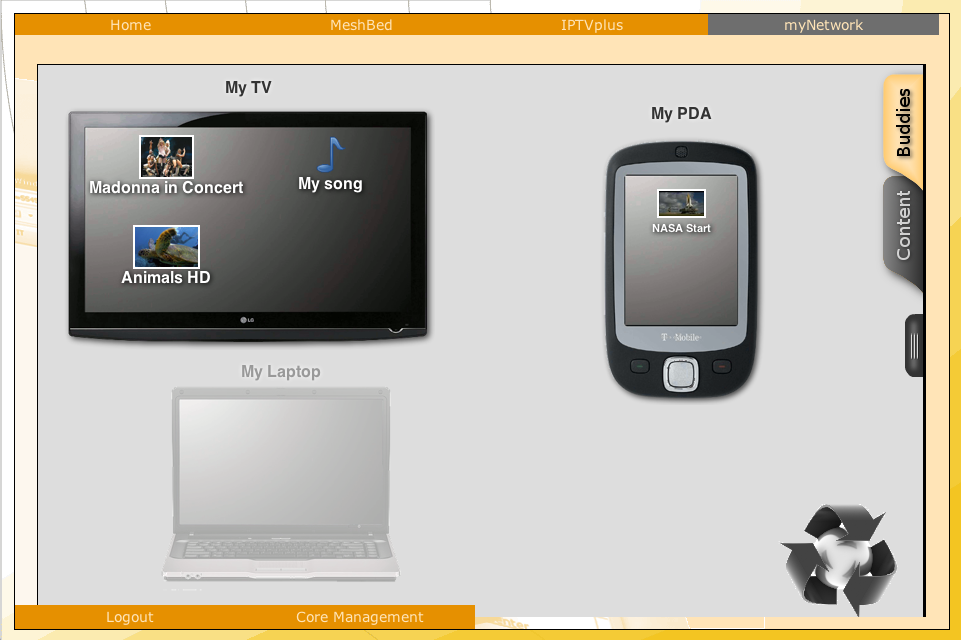
\includegraphics[width=\textwidth]{pnai-collapsed}
  \caption{PNAI interface with the collapsed sidebar}
  \label{fig:pnai-collapsed}
\end{figure}

Figure~\ref{fig:pnai-handover} describes several steps in the transferring of a session.
First the user drags the desired current session and drops it on another device.
Then a menu appears and the user clicks on the first option.
The interface notifies the backend so the video stops playing in the first container and starts playing in the second one.
While that happens, the user sees a popup with information about the status of the request.
When everything is finished, the popup disappears and the icon \emph{flies} to the target device.

\begin{figure}[htbp]
  \centering
  \subfigure[User drops the session onto another device, menu appears]{
    \label{fig:pnai-handover-menu}
    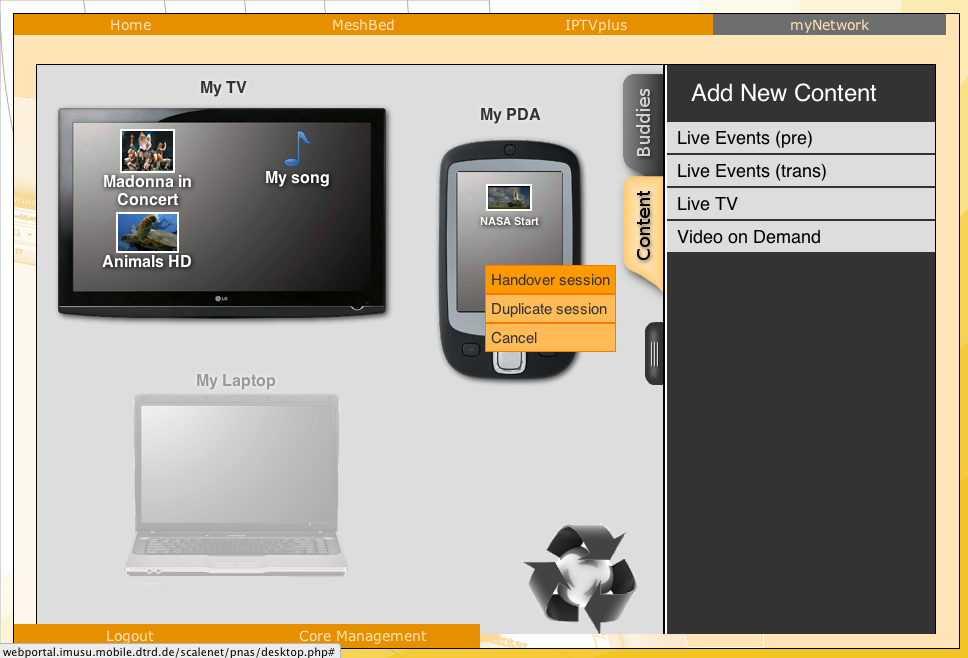
\includegraphics[width=0.75\textwidth]{pnai-handover}
  }
  \subfigure[A popup shows some information, session starts moving]{
    \label{fig:pnai-handovering}
    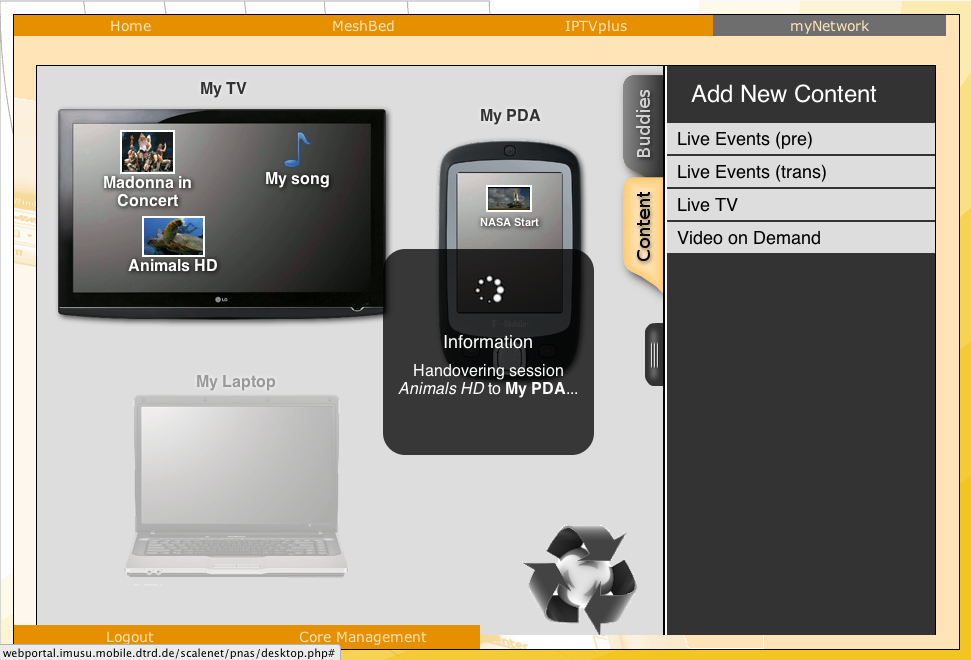
\includegraphics[width=0.75\textwidth]{pnai-handovering}
  }
  \subfigure[Content continues playing on the other device]{
    \label{fig:pnai-handovered}
    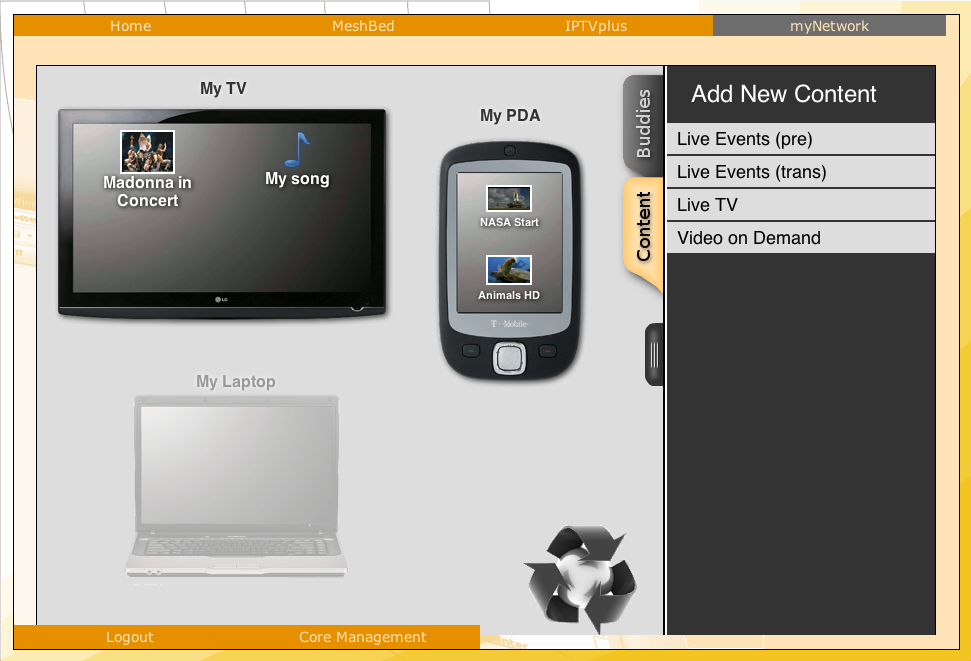
\includegraphics[width=0.75\textwidth]{pnai-handovered}
  }
  \caption{Transferring a session between two devices}
  \label{fig:pnai-handover}
\end{figure}

The process of buying new content can be triggered by clicking on any button that says \emph{Buy} (the session starts playing on the default device) or by dragging the icon from the content list to the desired device/buddy.
Since the buddy list is hidden, to select a buddy the user has to move the session to the \emph{Buddy} tab and then the buddy list appears.

Figure~\ref{fig:pnai-buy-content} contains some details of this process.
First we can see how the user is dragging the session to the device, and how the dragged session icon has a different appearance depending on its position.
The second detail is the popup window that appears to confirm the action.

\begin{figure}[htbp]
  \centering
  \subfigure[User starts dragging the icon, that is cloned with a dimmed appearance]{
    \label{fig:pnai-buy}
    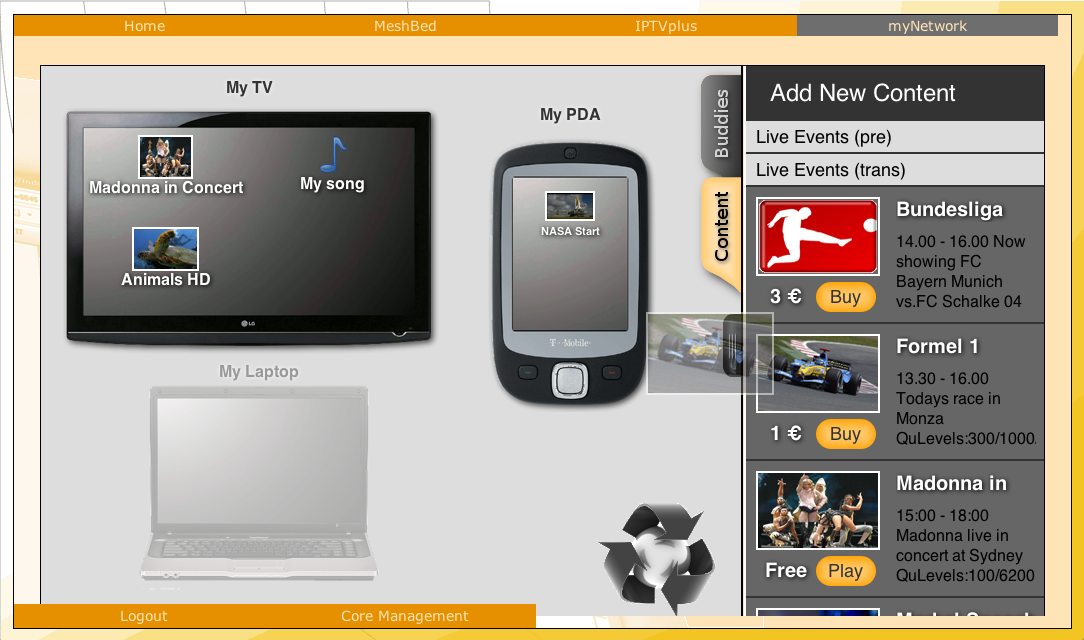
\includegraphics[width=0.9\textwidth]{pnai-buy}
  }
  \subfigure[When the icon reaches a valid device, the icon turns opaque]{
    \label{fig:pnai-buying}
    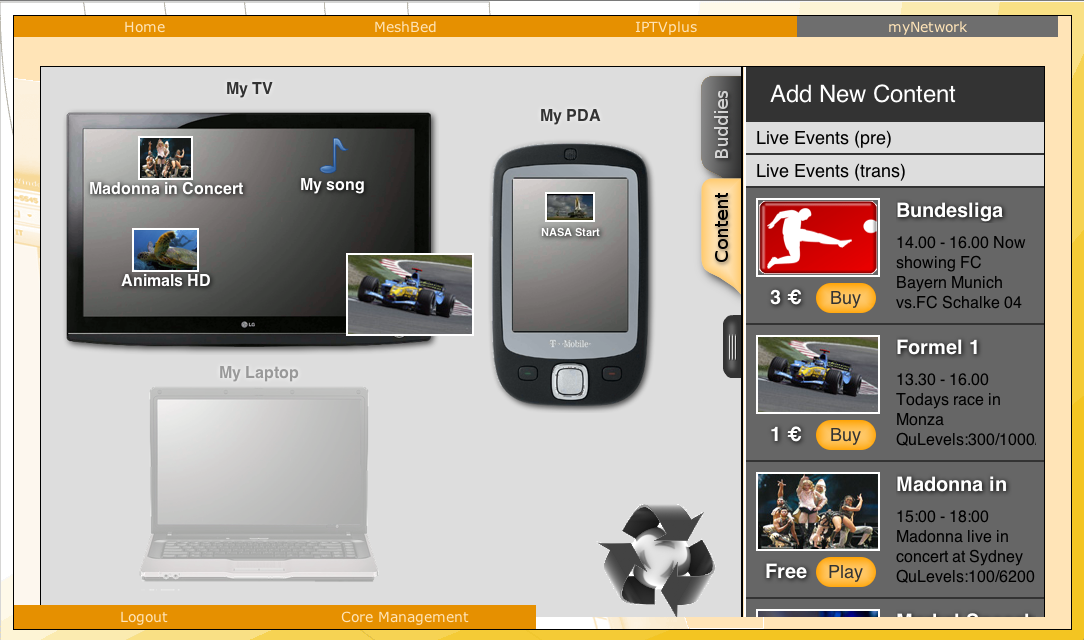
\includegraphics[width=0.9\textwidth]{pnai-buying}
  }
  \subfigure[Popup window that ask for confirmation]{
    \label{fig:pnai-bought}
    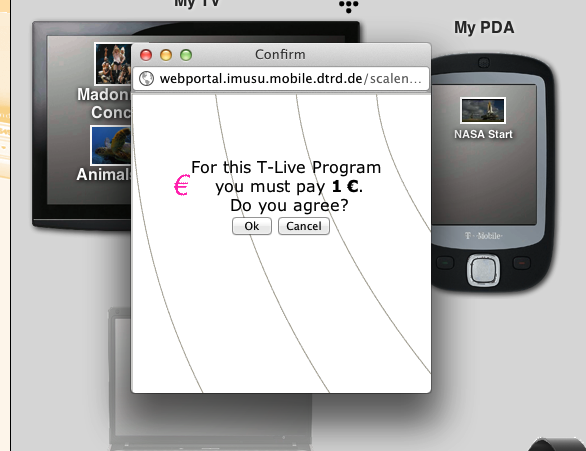
\includegraphics[width=0.5\textwidth]{pnai-bought}
  }
  \caption{Buying new content from the PNAI}
  \label{fig:pnai-buy-content}
\end{figure}

Sessions are deleted the same way as before, by dragging them from the device/buddy to the container.
Figure~\ref{fig:pnai-delete} exhibits another detail when deleting a session.
Notice that when the session icon reaches the trash, the trash icon recovers its true color.

\begin{figure}[htbp]
  \centering
    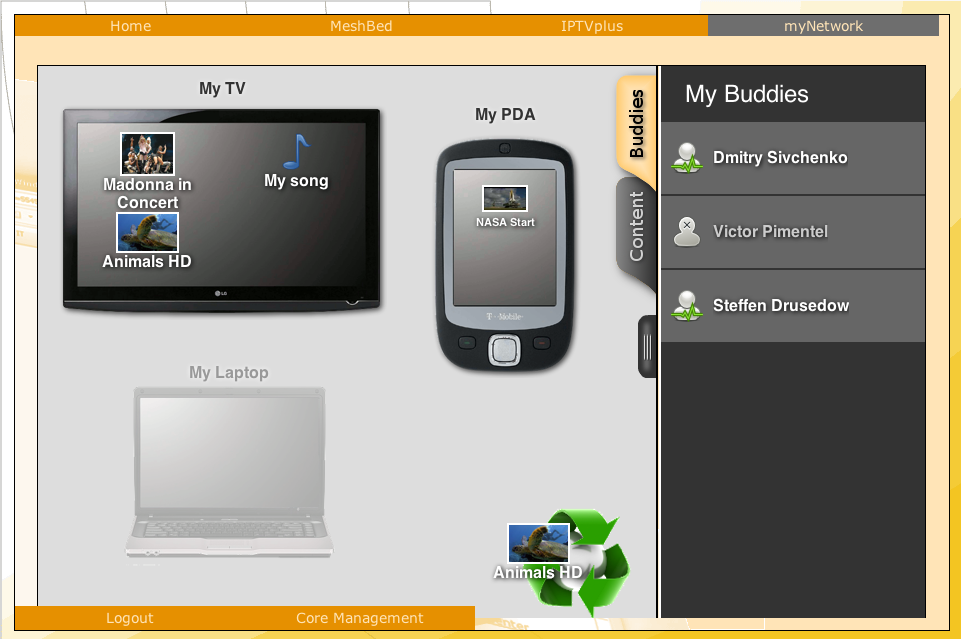
\includegraphics[width=\textwidth]{pnai-delete}
  \caption{Deleting a session in the new PNAI}
  \label{fig:pnai-delete}
\end{figure}

When the mouse stops on top of a container, two handles appear.
The one at the bottom left corner is for resizing that particular device.
Figure~\ref{fig:pnai-scale} shows how the device readapts to the required scale, resizing also the active sessions to the available space.

\begin{figure}[htbp]
  \centering
  \subfigure[When the mouse stops over a device, the handle appears]{
    \label{fig:pnai-scaling}
    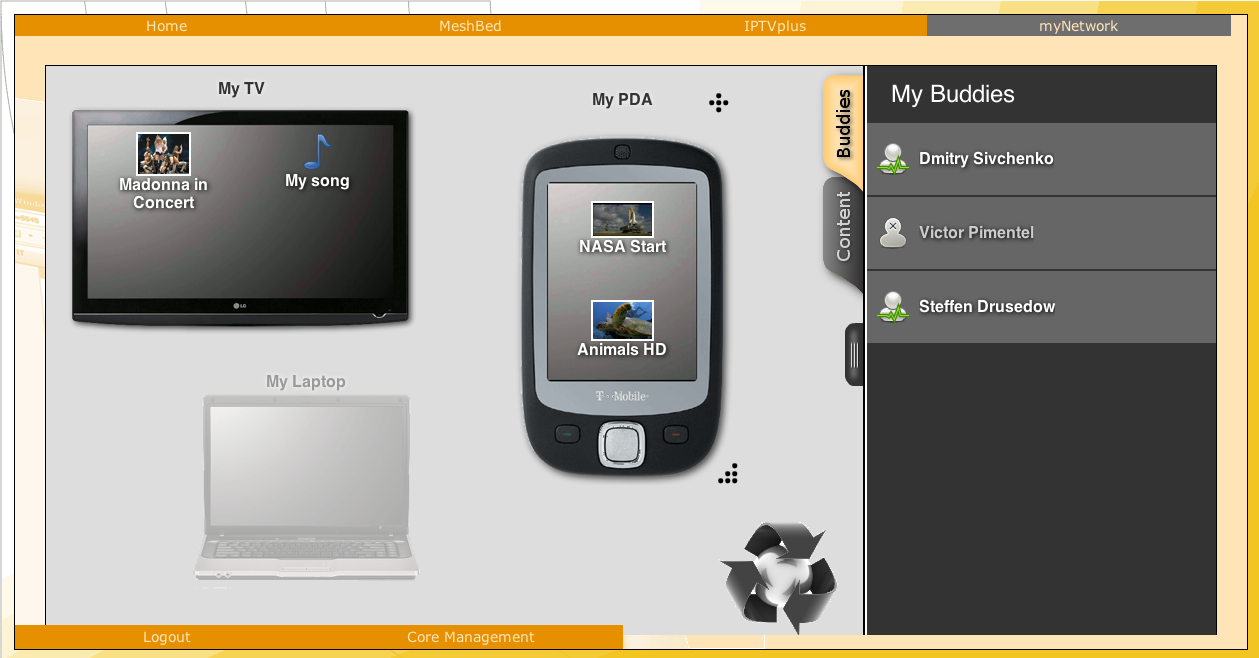
\includegraphics[width=\textwidth]{pnai-scaling}
  }
  \subfigure[If the user drags that handle, the device resizes according to the position of the mouse]{
    \label{fig:pnai-scaled}
    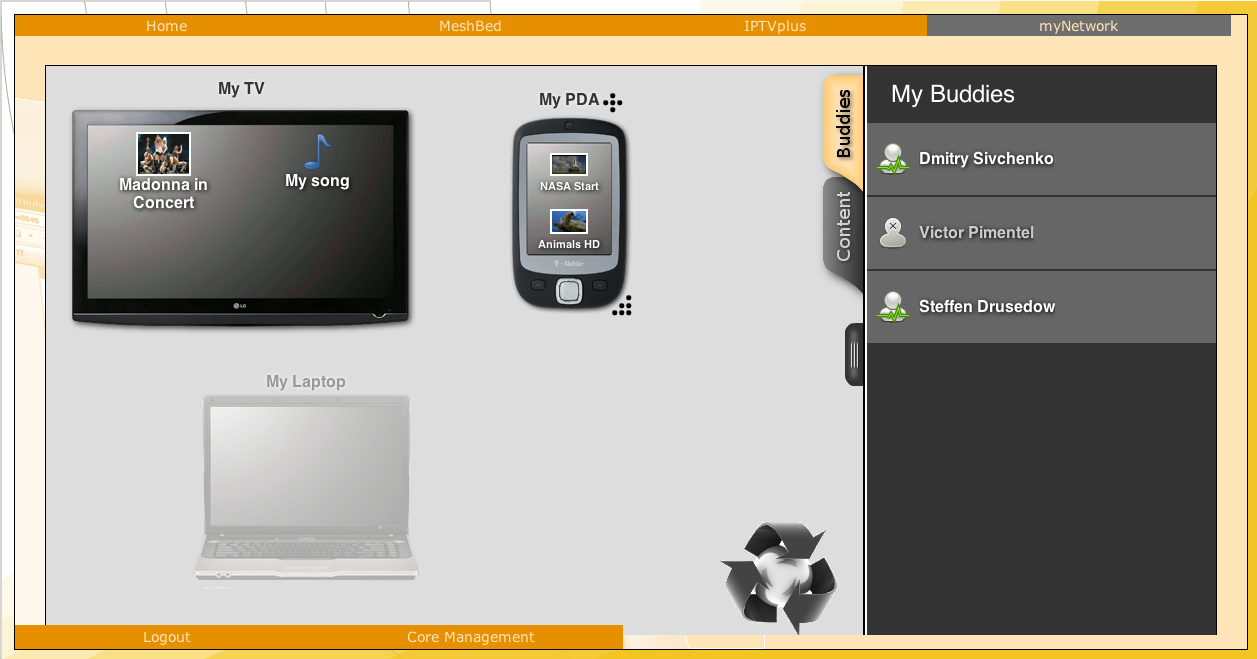
\includegraphics[width=\textwidth]{pnai-scaled}
  }
  \caption{Scaling a device in the PNAI}
  \label{fig:pnai-scale}
\end{figure}

The other handle appears in the top left corner and it is for moving the device to another position.
Figure~\ref{fig:pnai-move} shows how a device can be repositioned to anywhere in the left pane of the page.
There is also an interesting detail, as those figures also reveal how the sessions are drawn in the buddy list.

\begin{figure}[htbp]
  \centering
  \subfigure[When the icon reaches a valid device, the icon turns opaque]{
    \label{fig:pnai-moving}
    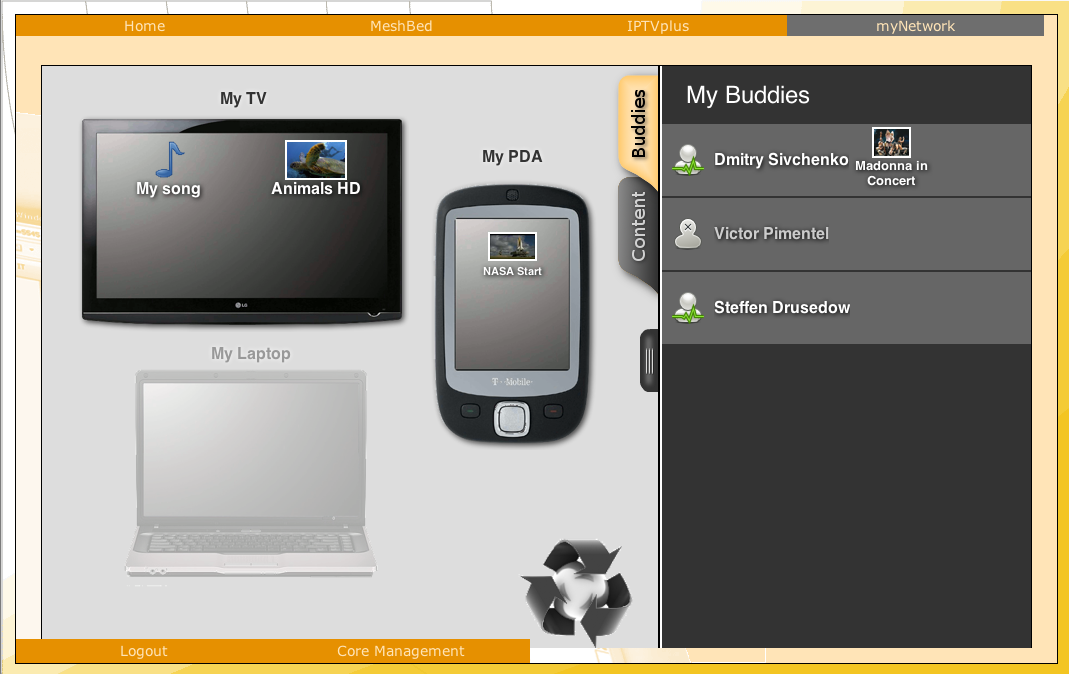
\includegraphics[width=\textwidth]{pnai-moving}
  }
  \subfigure[Popup window that ask for confirmation]{
    \label{fig:pnai-moved}
    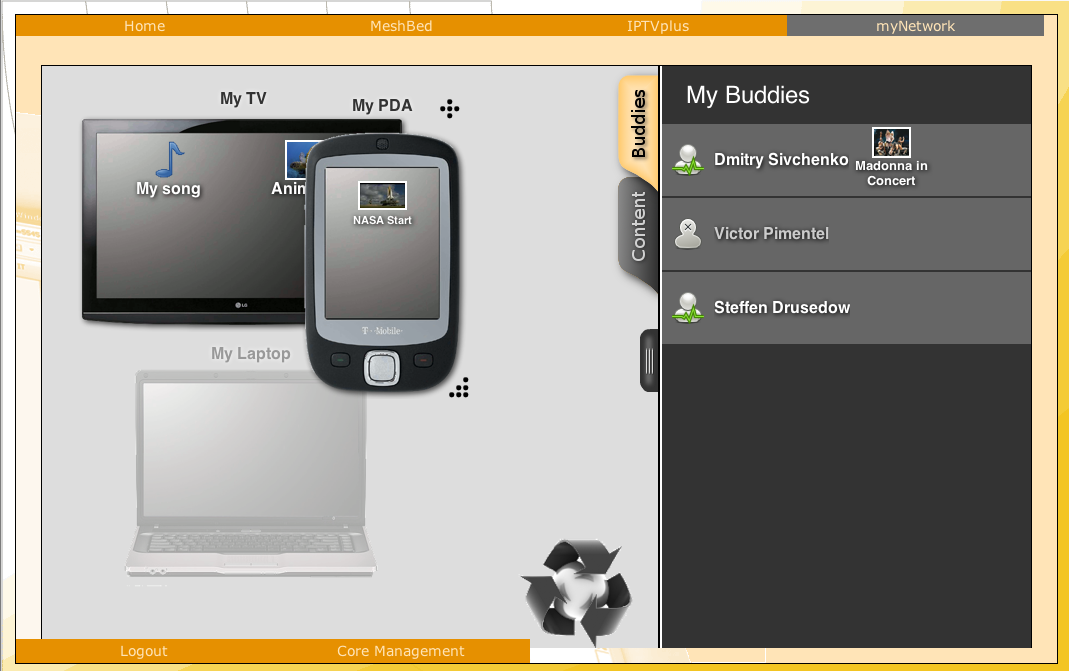
\includegraphics[width=\textwidth]{pnai-moved}
  }
  \caption{Buying new content from the PNAI}
  \label{fig:pnai-move}
\end{figure}

All this interface customizations are remembered the next time the user visits that page, using cookies to store that information.
Also, if the user resizes the window, the position and size of the devices are recalculated on the fly.

% subsection redesign (end)

\subsection{Mobile Design} % (fold)
\label{sub:mobile_design}

% subsection mobile_design (end)

% section interface_design (end)